%%%%%%%%%%%%%%%%%%%%%%%%%%%%%%%%%%%%%%%%%
% Beamer Presentation
% LaTeX Template
% Version 1.0 (10/11/12)
%
% This template has been downloaded from:
% http://www.LaTeXTemplates.com
%
% License:
% CC BY-NC-SA 3.0 (http://creativecommons.org/licenses/by-nc-sa/3.0/)
%
%%%%%%%%%%%%%%%%%%%%%%%%%%%%%%%%%%%%%%%%%

%----------------------------------------------------------------------------------------
%	PACKAGES AND THEMES
%----------------------------------------------------------------------------------------

\documentclass{beamer}

\mode<presentation> {

% The Beamer class comes with a number of default slide themes
% which change the colors and layouts of slides. Below this is a list
% of all the themes, uncomment each in turn to see what they look like.

%\usetheme{default}
%\usetheme{AnnArbor}
%\usetheme{Antibes}
%\usetheme{Bergen}
%\usetheme{Berkeley}
%\usetheme{Berlin}
%\usetheme{Boadilla}
%\usetheme{CambridgeUS}
%\usetheme{Copenhagen}
%\usetheme{Darmstadt}
%\usetheme{Dresden}
%\usetheme{Frankfurt}
%\usetheme{Goettingen}
%\usetheme{Hannover}
%\usetheme{Ilmenau}
%\usetheme{JuanLesPins}
%\usetheme{Luebeck}
\usetheme{Madrid}
%\usetheme{Malmoe}
%\usetheme{Marburg}
%\usetheme{Montpellier}
%\usetheme{PaloAlto}
%\usetheme{Pittsburgh}
%\usetheme{Rochester}
%\usetheme{Singapore}
%\usetheme{Szeged}
%\usetheme{Warsaw}

% As well as themes, the Beamer class has a number of color themes
% for any slide theme. Uncomment each of these in turn to see how it
% changes the colors of your current slide theme.

%\usecolortheme{albatross}
%\usecolortheme{beaver}
%\usecolortheme{beetle}
%\usecolortheme{crane}
%\usecolortheme{dolphin}
%\usecolortheme{dove}
%\usecolortheme{fly}
%\usecolortheme{lily}
%\usecolortheme{orchid}
%\usecolortheme{rose}
%\usecolortheme{seagull}
%\usecolortheme{seahorse}
%\usecolortheme{whale}
%\usecolortheme{wolverine}

\usepackage[utf8]{inputenc}
\usepackage[slovene]{babel}
\usepackage{physics}
\usepackage{amsmath}
\usepackage{bm}
\usepackage{amsfonts}
\usepackage{amssymb}
\usepackage{caption}
\usepackage{subcaption}
\usepackage{float}
\usefonttheme{professionalfonts} 

%\setbeamertemplate{footline} % To remove the footer line in all slides uncomment this line
%\setbeamertemplate{footline}[page number] % To replace the footer line in all slides with a simple slide count uncomment this line

%\setbeamertemplate{navigation symbols}{} % To remove the navigation symbols from the bottom of all slides uncomment this line
}

\usepackage{graphicx} % Allows including images
\usepackage{booktabs} % Allows the use of \toprule, \midrule and \bottomrule in tables

%----------------------------------------------------------------------------------------
%	TITLE PAGE
%----------------------------------------------------------------------------------------

\title[02-airbounce]{Airbounce} % The short title appears at the bottom of every slide, the full title is only on the title page

\author{FMF} % Your name
\institute[IPT] % Your institution as it will appear on the bottom of every slide, may be shorthand to save space
{
 \\ % Your institution for the title page
\medskip
\textit{} % Your email address
}
\date{\today} % Date, can be changed to a custom date

\begin{document}

\begin{frame}
\titlepage % Print the title page as the first slide
\end{frame}


%----------------------------------------------------------------------------------------
%	PRESENTATION SLIDES
%----------------------------------------------------------------------------------------

%------------------------------------------------


\begin{frame}
\frametitle{Official problem
statement}
When a Frisbee is thrown in a certain way it can be made to bounce in mid-air. Study the physics of this phenomenon.

\end{frame}

%------------------------------------------------

\begin{frame}
\frametitle{Stabilen frizbi}
\begin{itemize}
\item Frizbi zaradi vrtenja ohranja orientacijo.
\end{itemize}

\begin{figure}[H]
	\centering
	\begin{minipage}{.5\textwidth}
	  \centering
	  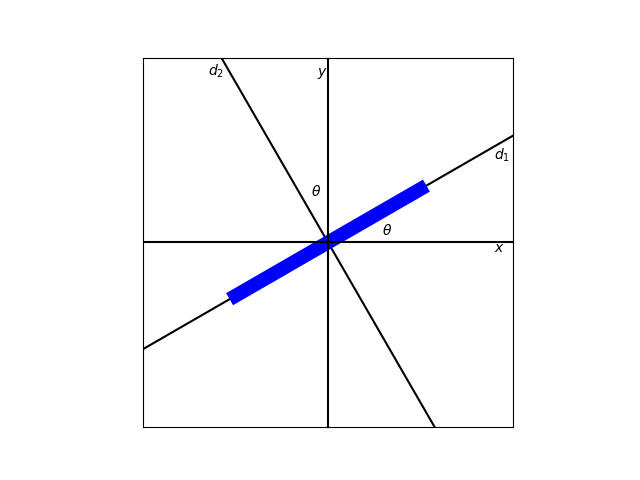
\includegraphics[width=6cm]{graf_osi.png}
	  \captionof{figure}{Graf osi, koordinatni sistem N}
	\end{minipage}%
	\begin{minipage}{.5\textwidth}
	  \centering
	  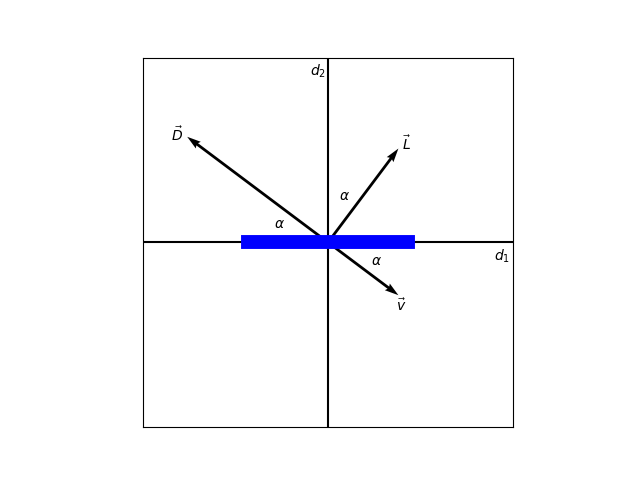
\includegraphics[width=6cm]{osi_frisbeeja.png}
	  \captionof{figure}{Koordinatni sistem frizbija D}
	\end{minipage}
\end{figure}

\end{frame}

%------------------------------------------------

\begin{frame}
V sistemu frizbija (D):
\begin{gather}
L = \dfrac{1}{2} A \rho C_L v^2 \qquad D = \dfrac{1}{2} A \rho C_D v^2\\
C_L = C_{L0} + C_{L \alpha} \alpha \qquad C_D = C_{D0} + C_{D \alpha} \alpha^2\\
K = \dfrac{A \rho}{2 m} \qquad \tan \alpha = \dfrac{-v_2}{v_1}\\
\bm L = m K v^2 C_L \mqty(\sin \alpha \\ \cos \alpha) = m K v^2 C_L \mqty(-v_2 \\ v_1\\)\\
\bm D = m K v^2 C_D \mqty(-\cos \alpha \\ \sin \alpha) = m K v^2 C_D \mqty(-v_1 \\ -v_2\\)\\
\bm F_{\bm g} = - m g  \mqty(\sin \theta \\ \cos \theta)
\end{gather}
\end{frame}

%------------------------------------------------

\begin{frame}
\begin{gather}
m \bm a = \bm L + \bm D + \bm F_{\bm g}\\
v = \sqrt{v_1^2 + v_2^2}\\
a_1 = -K (C_{L0} + C_{L \alpha} \alpha) v v_2 - K (C_{D0} + C_{D \alpha} \alpha^2) v v_1 - g \sin \theta\\
a_2 = K (C_{L0} + C_{L \alpha} \alpha) v v_1 - K (C_{D0} + C_{D \alpha} \alpha^2) v v_2 - g \cos\theta
\end{gather}
Rešimo: \(d_1, d_2, v_1, v_2 \).\\
Zarotiramo v N sistem.
\begin{gather}
R = \mqty(\cos \theta & -\sin \theta \\ \sin \theta & \cos \theta)\\
\mqty(x \\ y)_N = R \mqty(d_1 \\ d_2)_D\\
\mqty(v_x \\ v_y)_N = R \mqty(v_1 \\ v_2)_D
\end{gather}
\end{frame}

%------------------------------------------------

\begin{frame}
\frametitle{Koeficienti lift-a in drag-a.}
\[C_L = C_{L0} + C_{L \alpha} \alpha \qquad C_D = C_{D0} + C_{D \alpha} \alpha^2\]\\
\begin{itemize}

\item Za koeficient drag-a $C_D$ cutoff, ko doseže $C_D$ vrednost diska, ki je pravokoten na hitrost.

\item Za koeficient lift-a $C_L$, cutoff pri stall angle.
\end{itemize}
\begin{figure}[H]
	\centering
	  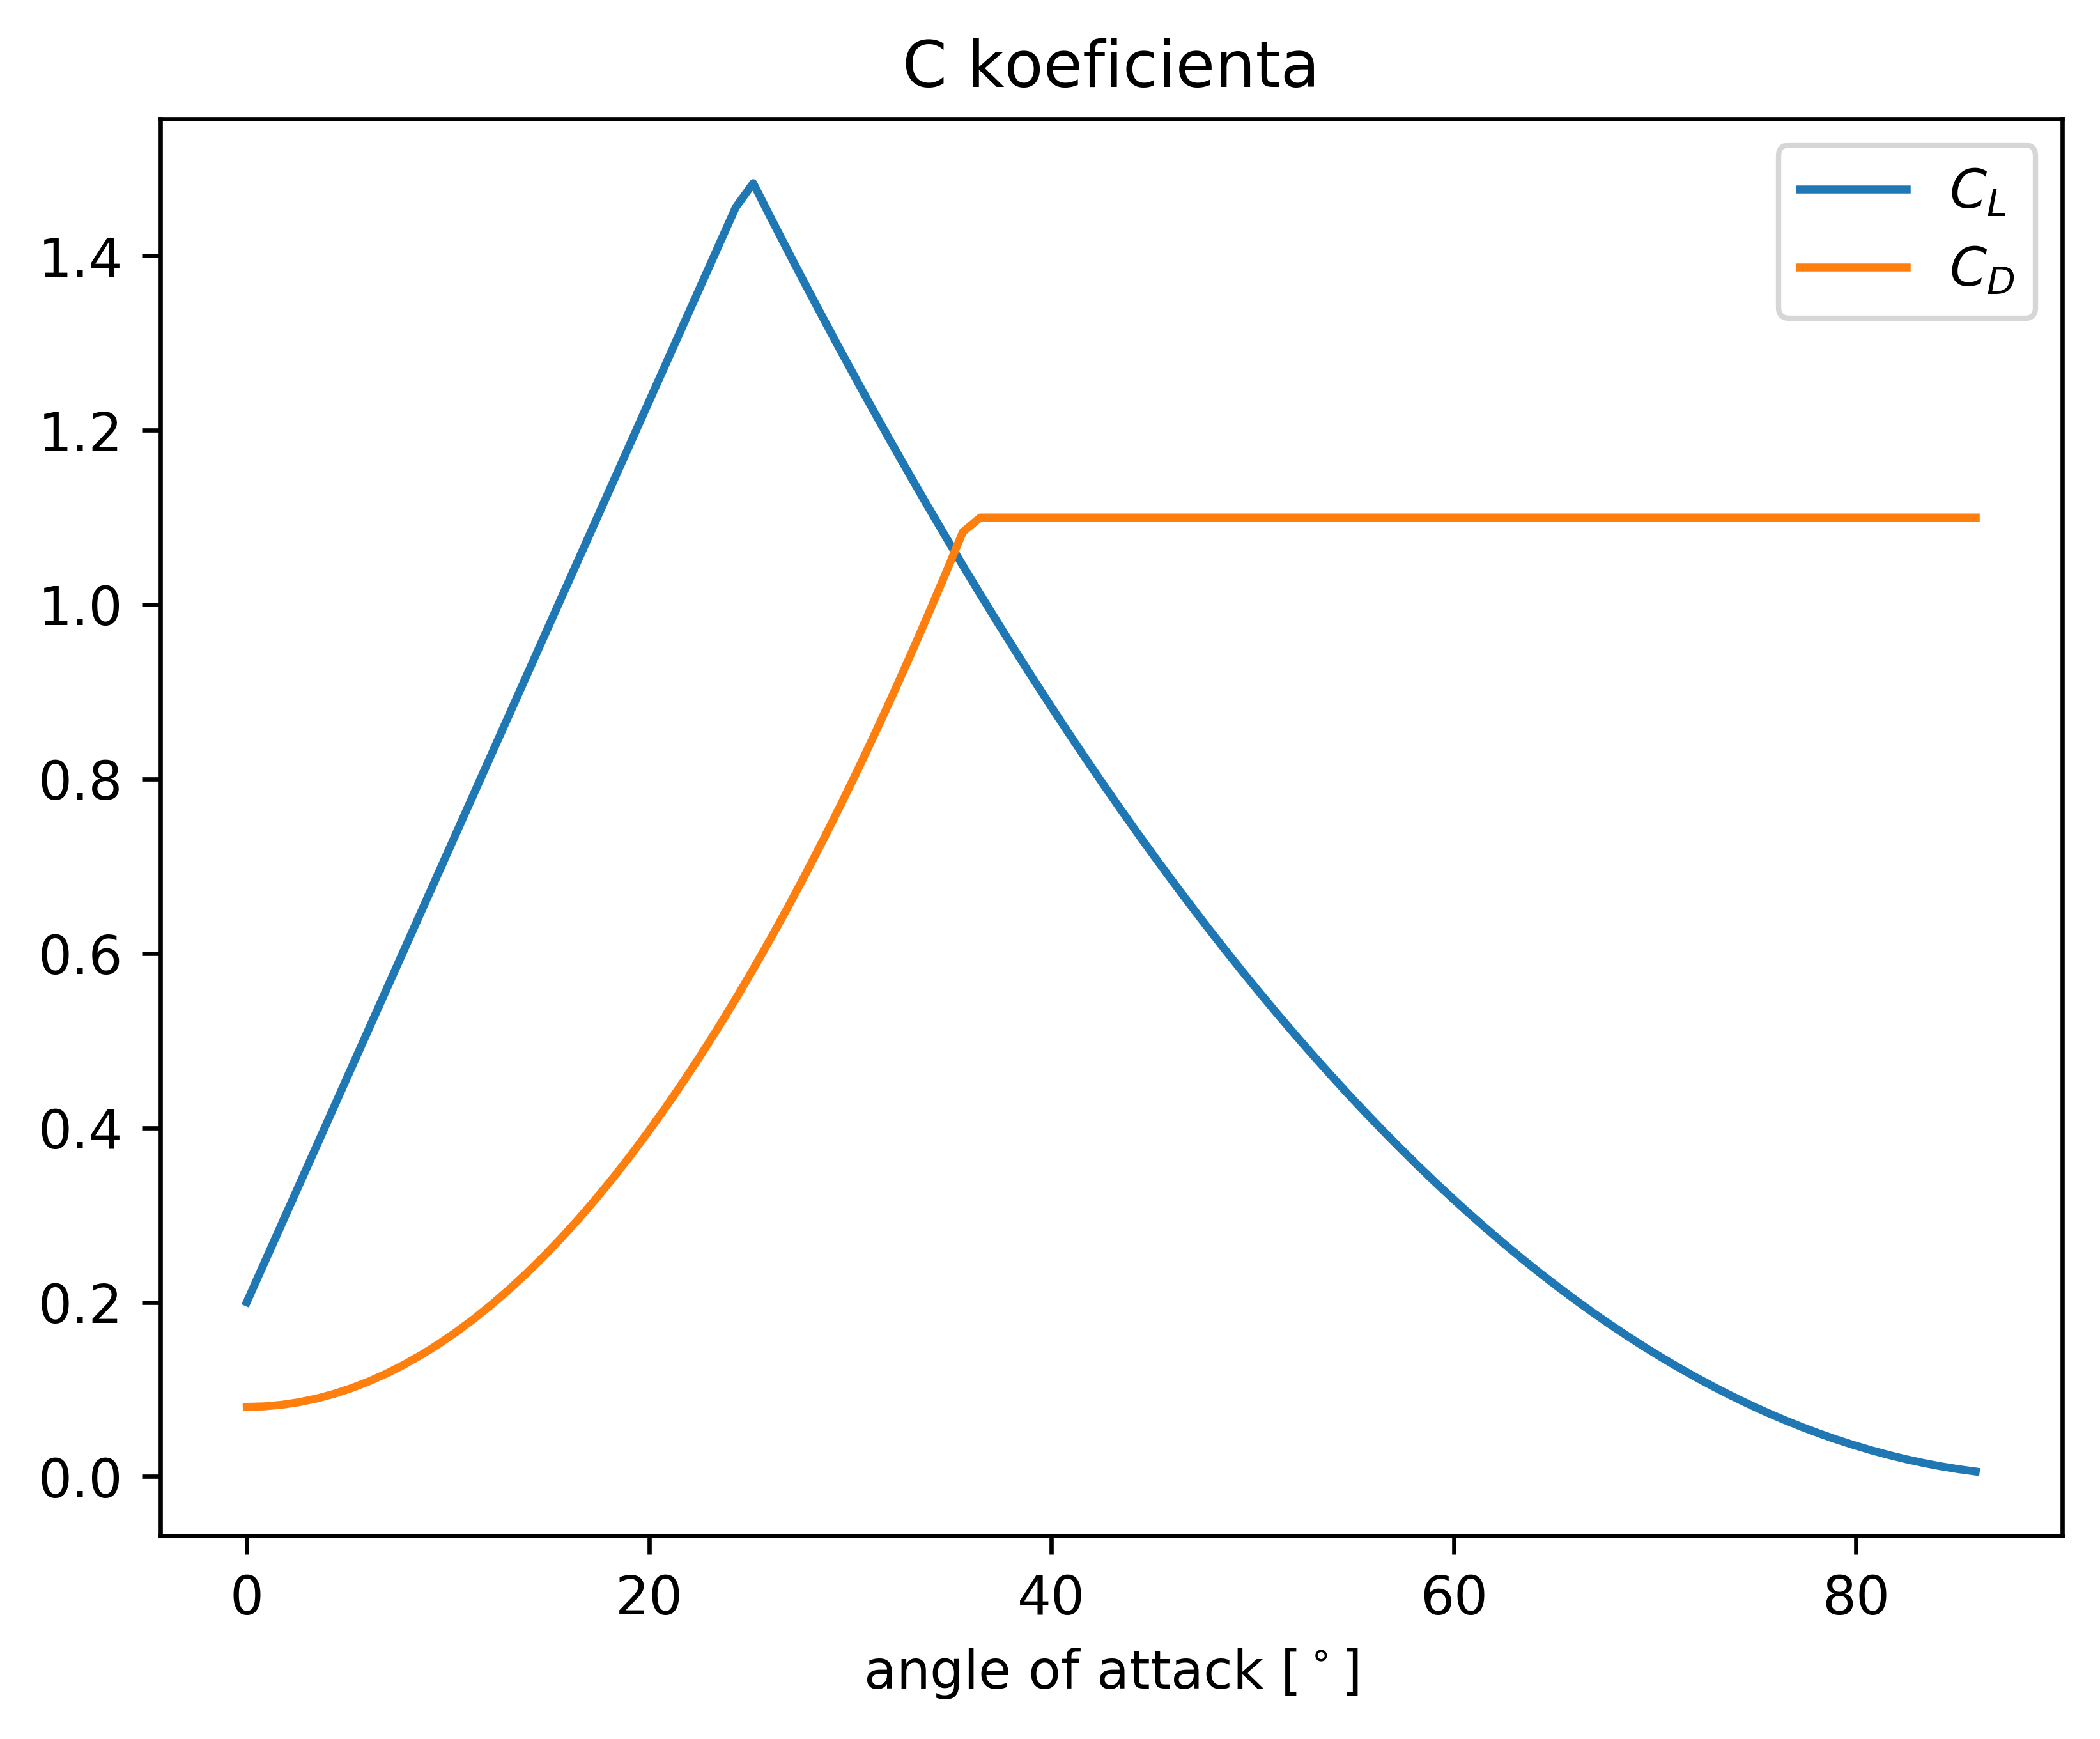
\includegraphics[width=6cm]{koeficienta_cutoff.png}
\end{figure}
\end{frame}

%------------------------------------------------

\begin{frame}
\frametitle{Met: različni začetnimi koti.}
Začetna hittrost = (15, -8) m/s
\begin{figure}[H]
	\centering
	  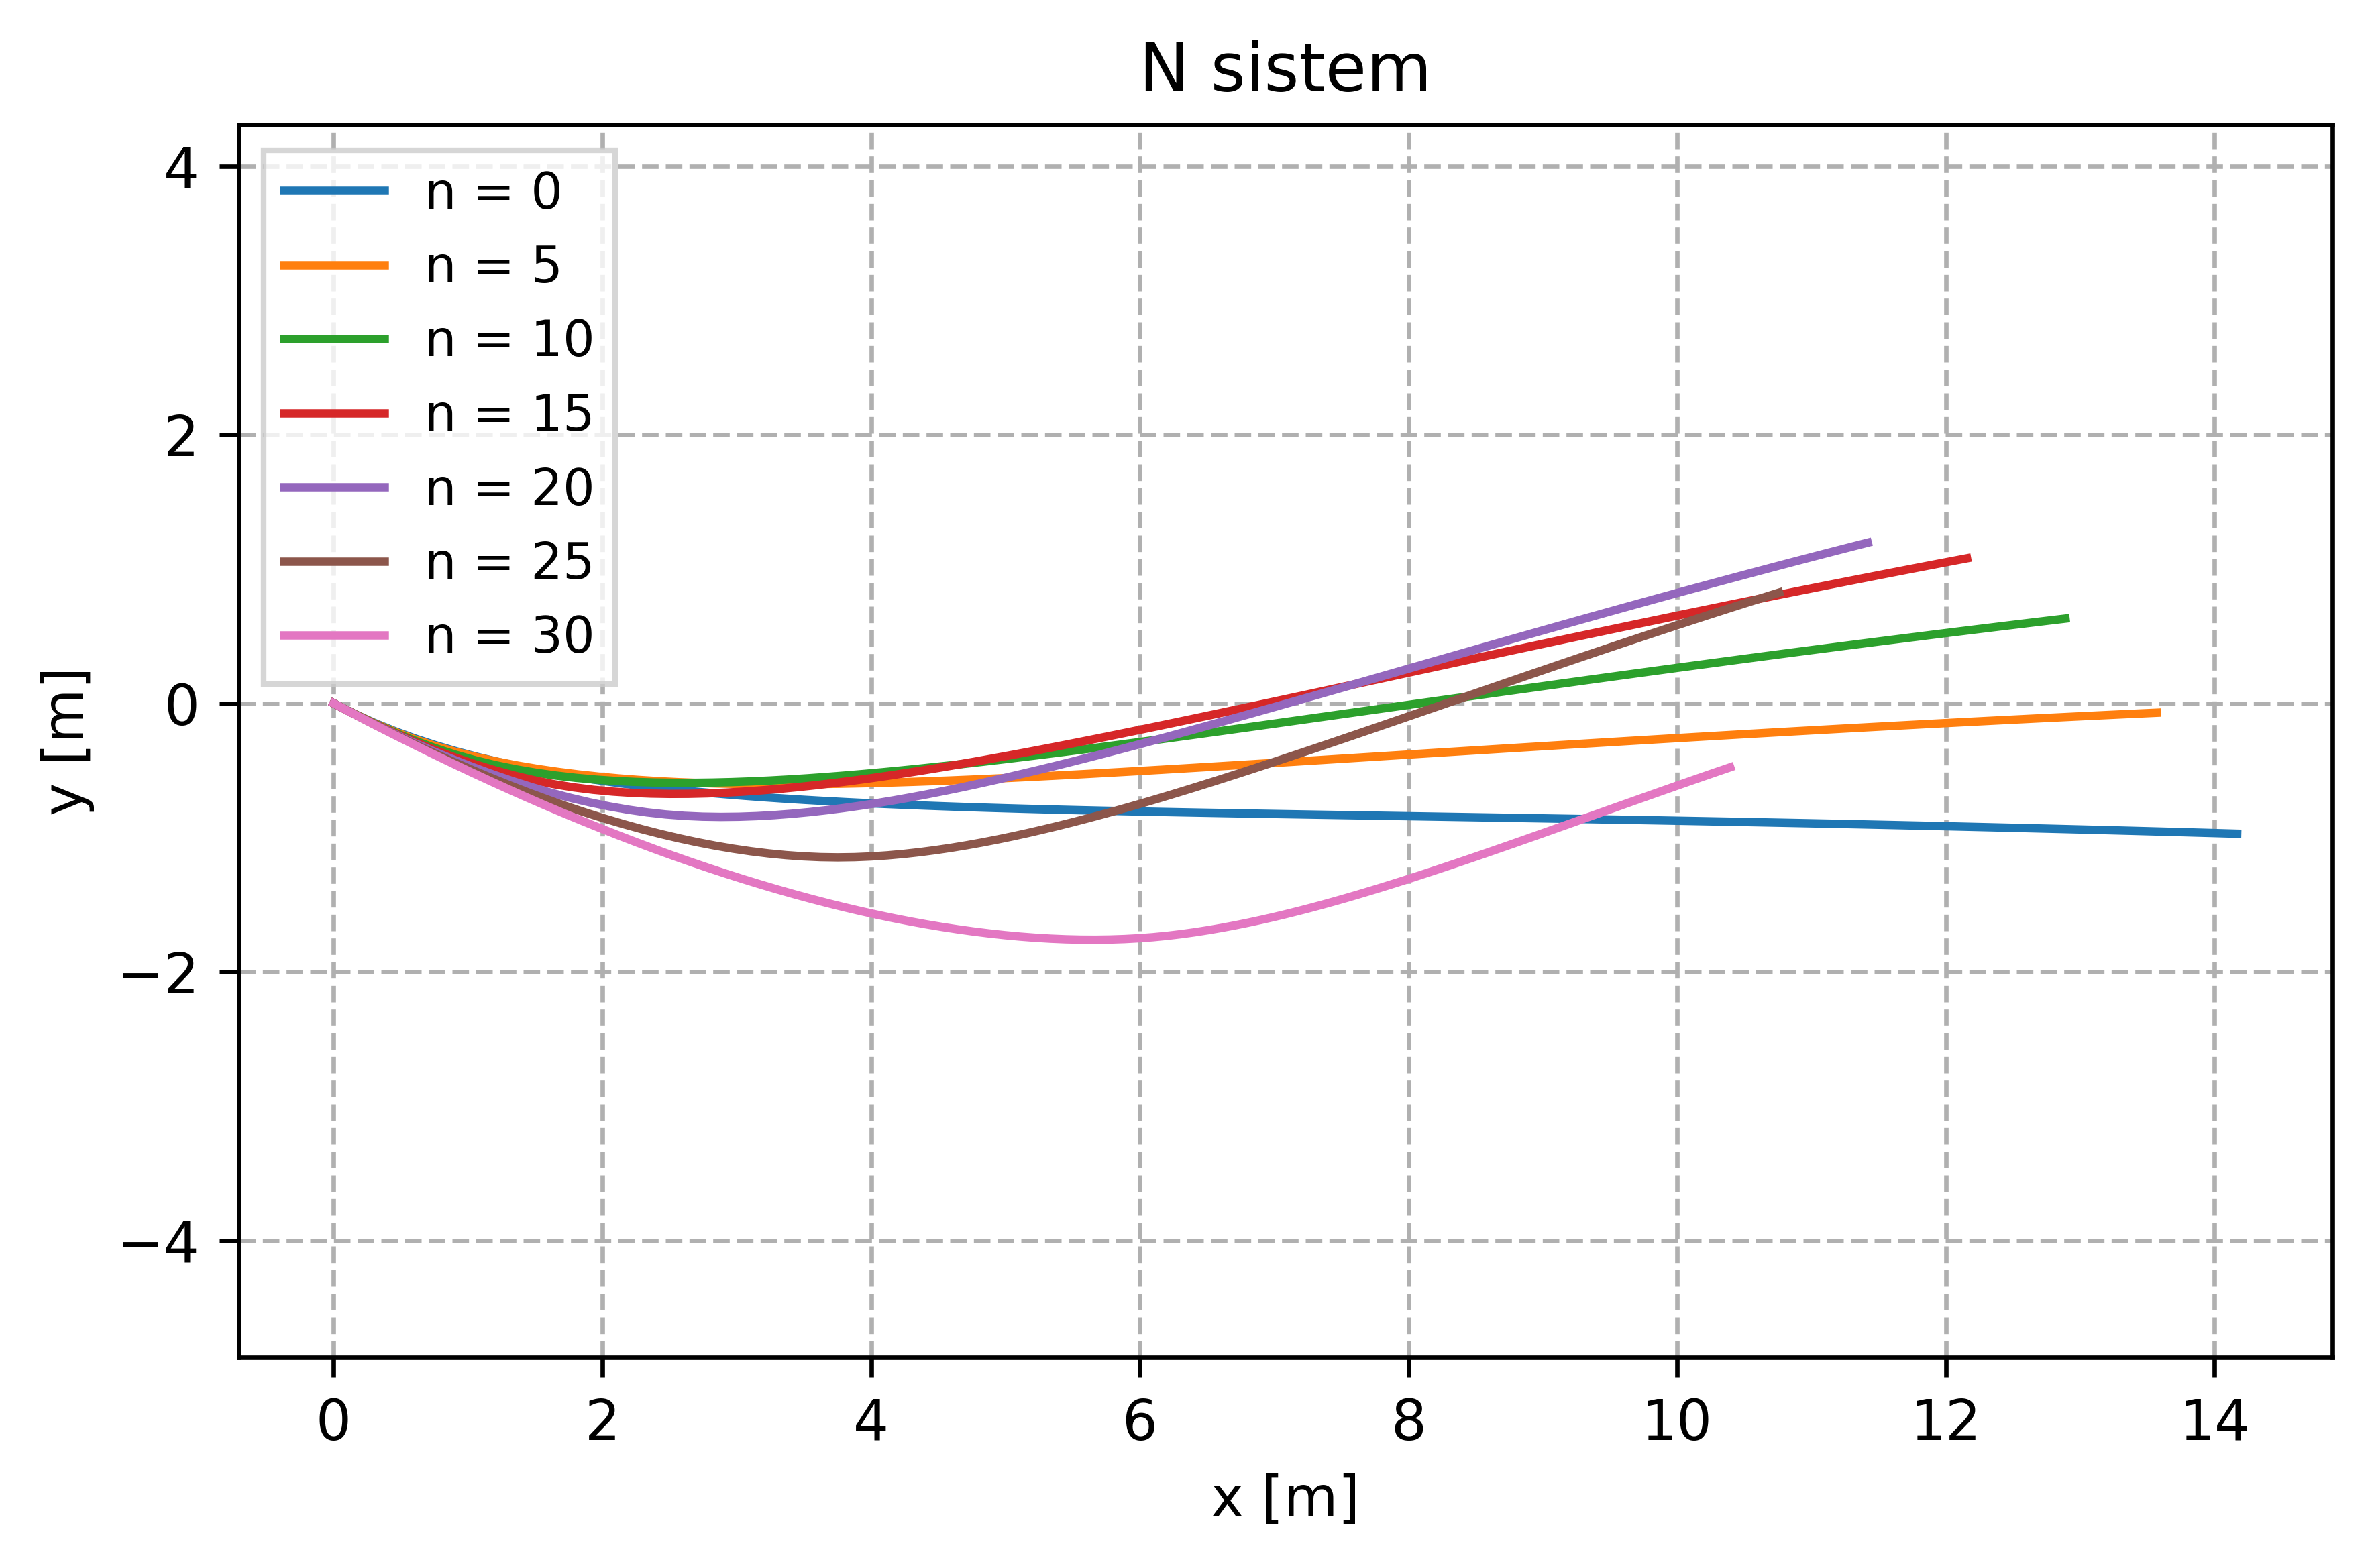
\includegraphics[width=9cm]{med_razlicni_koti.png}
\end{figure}
\end{frame}

%------------------------------------------------

\begin{frame}
\frametitle{Problemi}
\begin{itemize}
\item Pri mojem metu ni stabilen.
\item Wobbling frisbee.
\end{itemize}
\end{frame}

%------------------------------------------------
\begin{frame}
\frametitle{Plan za naprej}
\begin{itemize}
\item Naučim se boljši met, da ni treba simulirati wobble-a.
\item Če se ujema s simulacijo: v brezdimenzijsko, fazni diagram kdaj se pojavi je airbounce...
\end{itemize}
\end{frame}

%------------------------------------------------

\end{document} 